\documentclass[12pt]{article}
\usepackage[utf8]{inputenc}
\usepackage[estonian,english]{babel}
\usepackage[a4paper]{geometry}
\usepackage{array}
\usepackage{hyperref}

\usepackage{amsmath}
\usepackage{amsthm}

\usepackage{todonotes}
\usepackage{tikz}
\usetikzlibrary{backgrounds}

\newcommand{\TODO}{\todo[inline]}
\newcommand{\nstat}{\mathrm{nstat}}
\newcommand{\occu}{\mathrm{occu}}
\newcommand{\go}{\mathrm{go}}
\newcommand{\cont}{\mathrm{cont}}
\newcommand{\stp}{\mathrm{stop}}
\newcommand{\lift}{\mathrm{lift}}
\newcommand{\drop}{\mathrm{drop}}
\newcommand{\edg}{\mathrm{edg}}
\newcommand{\W}{\mathcal{W}}
\newcommand{\Wm}{\mathcal{W}_\mathrm{move}}
\newcommand{\Wmc}{\mathcal{W}_\mathrm{mc}}
\newcommand{\Wl}{\mathcal{W}_\mathrm{lift}}
\newcommand{\Wd}{\mathcal{W}_\mathrm{drop}}
\newcommand{\D}{\mathcal{D}}
\newcommand{\T}{\mathcal{T}}
\newcommand{\td}{\delta}
\newcommand{\Tn}{\overline{\T}}
\newcommand{\V}{\mathcal{V}}
\newcommand{\E}{\mathcal{E}}
\newcommand{\N}{\mathcal{N}}
\newcommand{\A}{\mathcal{A}}
\newcommand{\B}{\mathcal{B}}

\newcommand{\uw}{\mathrm{uWhat}}
\newcommand{\um}{\mathrm{uMore}}
\newcommand{\ul}{\mathrm{uLess}}
\newcommand{\vl}{\mathrm{vLess}}
\newcommand{\getMC}{\mathrm{getMC}}
\newcommand{\remMC}{\mathrm{remMC}}
\newcommand{\addMC}{\mathrm{addMC}}
\newcommand{\goOrCont}{\mathrm{goOrCont}}
\newcommand{\IF}[1]{\text{if}\ #1 \colon}
\newcommand{\away}{\mathrm{away}}
\newcommand{\more}{\mathrm{more}}

\newcommand{\Dn}{North}
\newcommand{\De}{East}
\newcommand{\Ds}{South}
\newcommand{\Dw}{West}

\newcommand{\stat}[1]{\text{\bf #1}}


\newtheorem{theorem}{Theorem}
\newtheorem{lemma}{Lemma}
\begin{document}
\thispagestyle{empty}
\begin{center}

\large
UNIVERSITY OF TARTU\\[2mm]
Institute of Computer Science\\
Computer Science Curriculum\\[2mm]

\vspace{25mm}

\Large Karl Tarbe

\vspace{4mm}

\huge \myTitle

\vspace{20mm}

\Large Master's Thesis (30 ECTS)

\end{center}

\vspace{2mm}

\begin{flushright}
 {
 \setlength{\extrarowheight}{5pt}
 \begin{tabular}{r l} 
  \sffamily Supervisor: & \sffamily Dr. Dirk Oliver Theis
 \end{tabular}
 }
\end{flushright}

\vfill
\centerline{Tartu 2016}

\noindent\textbf{\large \myTitle}
\vspace*{3ex}
{\flushleft{\textbf{Abstract:}} }
As parking becomes a more and more complex problem with the number of cars and
city density, more complex solutions can be used to rectify it. One of possible
solutions for parking is automated valet parking, where cars are not driven to
parking place by humans but are carried by specially designed robots. Such
solution presents us many possible optimization problems, one of which is
addressed in this work using Integer Programming models, that can by solved
using off-the-shelf solvers. We look at a specific possible implementation of
automated valet parking and succesfully design an Integer Programming model to
solve it. Existing theoretical results have shown that even simplified cases of
the problem can be APX-hard~\cite{calinescu2008reconfigurations}. Using Gurobi,
optimal solution was found for sample cases. The model is compared to another
integer programming model from Algorithms and Theory research group, which
provides comparison and verification for the model performance.

\vspace*{3ex}
{\flushleft{\textbf{Keywords:} integer programming,
\vspace*{3ex}

\noindent\textbf{CERCS:} P170 Computer science, numerical analysis, systems,
control 
\vspace*{3ex}
\newpage
%\selectlanguage{estonian}
\noindent\textbf{\large \myTitlE}
\vspace*{3ex}

{\flushleft{\textbf{Lühikokkuvõte:}} }
Kuna parkimine on autode hulga suurenemisega ja linnastumise tihenemisega üha
keerulisem ja keerulisem probleem, muutub selle kõrgtehnoloogiline lahendamine
otstarbekaks. Üks pakutud lahendus on automaatparkla, kus autodega ei sõideta
oma parkimiskohta, vaid autod toimetatakse parkimiskohta ja tagasi
spetsiaalsete robotite poolt. Selline kõrgtehnoloogiline lahendus annab meile
palju erinevaid optimiseerimise ülesandeid ja võimalusi, millest ühte
konkreetset käsitleme käesolevas töös kasutades täisarv optimiseerimise
mudeleid, mida saab lahendada juba eksisteerivate analüütiliste lahendajatega.
Käesolevas töös käsitletakse ühte kindlat võimalikku automaatparkla
implementatsiooni ja edukalt tuletatakse täisarv planeerimise mudel selle
lahendamiseks. Varasemad teoreetilised tulemused on näidanud, et isegi
lihtsustatud variandid sellest probleemist saavad olla
APX-keerukusega~\cite{calinescu2008reconfigurations}. Kasutades Gurobi
lahendajat leiti optimaalne lahendus näidis juhtude jaoks. Mudelit võrreldi
teise täisarv planeerimise mudeliga algoritmide ja teooria teadusgruppist, mis
andis kindlust ja võrdlusmaterjali mudeli toimimisele.

\vspace*{3ex}
{\flushleft{\textbf{Keywords:} integer programming,
%\noindent\textbf{Võtmesõnad:} täisarvuline planeerimine
\vspace*{3ex}

\noindent\textbf{CERCS:} P170 Arvutiteadus, arvutusmeetodid, süsteemid,
juhtimine (automaatjuhtimisteooria)
\vspace*{3ex}
%\selectlanguage{english}

\listoftodos
\tableofcontents
\section{Introduction}
It does not take a scientific paper to see that the number of cars on our
streets has increased. This creates a need for more parking places. It is
common for shopping centers and other public places with lots of quests to have
large parking lots or even parking houses. However, finding a parking space
still is a frustrating experience for the drivers. Some fancy places have valet
parking. Valet parking is rare in Estonia, but it is quite common in North
America. Valet parking means that the driver does not have to self-park and a
valet will park their car.

Since the industrial revolution when a lot of manufacturing by hand was replaced
by automation, other manual tasks are handed over to machines. One of those
tasks is valet parking. Instead of a human valet, there is a parking robot that
carries your car to a free parking space. In the system explored in this
thesis, drivers will stop their cars on a special platform. A parking robot can
freely move under those platforms and also can lift the platform up from the
ground and carry it to another place with the drivers car still on the
platform. For a driver the experience should be very similar to regular valet
parking: driver stops near the door and does not need to worry about parking,
after visiting the venue the driver can notify the system and will have their
car brought back to them.
\TODO{Write about a more concrete system.}
\subsection{The problem}
\TODO{Some pictures of actual robots?}
In an automated valet parking system, the software has to choose which of
possibly many parking robots will service the incoming parking or car retrieval
request, it will also need to figure out a path for the robots. Regular car
parks have passageways, so that no car is parked in a way that would block
other cars from entering or exiting. In an automated system we do not need
passageways, because blocking cars can be lifted and moved out of the way.
It is important that the time taken to retrieve cars is minimized, otherwise
drivers feel like they are wasting their time, waiting for their car. In a car
park without passageways, the parking robots have to be cooperative and cannot
do path planning as independent agents like in~\cite{wurman2008coordinating}.

There are a lot of optimization problems in a automated parking system
described. We chose to tackle a sub-problem: given a initial configuration of
robots and cars in the system and a terminal configuration, find the best
sequence of actions for robots to transform the initial configuration into the
terminal configuration. Note that best in this case means mostly shortest time,
but we might also want to avoid unneeded actions because they waste energy and
moving parts wear.

\TODO{write about other approaches}

We chose to specify the problem as an integer programming model optimization
problem. Unlike approximation algorithms, integer programming will give us a
strong guarantee that the solution found is in fact optimal.

\subsection{More specific problem description}
The parking robot can move either forwards, backwards or sideways. The length of
the parking space is 6 meters, and it is 3 meters wide. The robots have smaller
dimensions. Every action takes some time. Lifting a car takes 9 seconds,
lowering it will take 3 seconds. The speed of the robot is 2 meters per second,
when not carrying a car, and 1 meter per second, when loaded. Robots needs time
to accelerate and de-accelerate. Changing the direction takes 3 seconds.

The last paragraph describes the information we received. However there is still
some room to interpret the acceleration of the robot. It is said that changing
direction takes 3 seconds. The interpretation we used, is that it takes 1.5
seconds to stop a robot moving at it's maximum speed. And another 1.5 seconds to
accelerate it to maximum speed in another direction. Maximum speed depends on
whether the robot is carrying a car or not, however it makes sense that the
acceleration of robot can be greater, when the mass is lower. Meaning that a
heavy loaded robot can accelerate to speed 1 meter per second and that the empty
robot can accelerate to speed 2 meters per second in the same time. It might
help to see~\autoref{fig:changedir}.

\begin{figure}[h]
    \begin{center}
        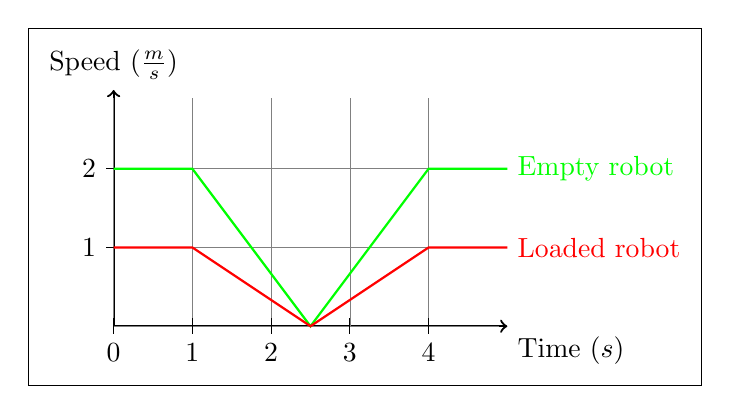
\begin{tikzpicture}[show background rectangle]
\draw[thick,->] (0,0) -- (0,3) node[above] {Speed ($\frac{m}{s}$)};
\draw[thick,->] (0,0) -- (5,0) node[below right] {Time ($s$)};
\draw[very thin, gray] (0,0) grid (4.9,2.9);

\foreach \x in {0,...,4}
    \draw (\x,0.1) -- (\x,-0.1) node [below] {\x};

\foreach \y in {1,...,2}
    \draw (0.1,\y) -- (-0.1,\y) node [left] {\y};

% path
\draw[thick, green] (0,2) -- (1,2) -- (2.5,0) -- (4,2) -- (5,2) node[right] {Empty robot};
\draw[thick, red] (0,1) -- (1,1) -- (2.5,0) -- (4,1) -- (5, 1) node[right] {Loaded robot};
\end{tikzpicture}
\TODO{Maybe improve this figure}

        \caption{This diagram serves as an illustration for the interpretation of
            time it takes to change direction. The direction of movement can change
            instantaneously, when speed is 0. Change of direction is not explicitly shown on
            this graph.}
        \label{fig:changedir}
    \end{center}
\end{figure}

It is assumed that car park is a grid of of parking spaces. We define a set of
directions as $\D = \{\Dn, \De, \Ds, \Dw\}$. A parking place in the $\Dn$ -
$\Ds$ dimension is 6 meters long, and in the $\De$ - $\Dw$ dimension is 3
meters wide. Note that the directions defined here do not have to correspond to
geographical directions.

After those definitions we can say that an empty robot can go to adjacent space
in the $\Dn$ or $\Ds$ direction in 4.5 seconds. Empty robot can go to adjacent
space in the shorter dimension in 3 seconds. A loaded robot needs 7.5 seconds
to reach adjacent parking space in the longer dimension and 4.5 seconds for
shorter dimension. Speed versus time graph of all of those movements is
on~\autoref{fig:moving times}, the area under those lines is equal to the
dimensions of the parking space.
\begin{figure}[h]
    \begin{center}
        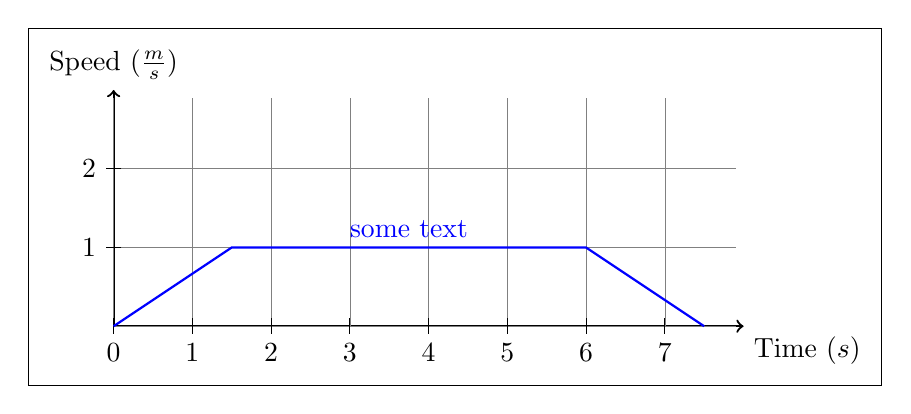
\begin{tikzpicture}[show background rectangle]
\draw[thick,->] (0,0) -- (0,3) node[above] {Speed ($\frac{m}{s}$)};
\draw[thick,->] (0,0) -- (8,0) node[below right] {Time ($s$)};
\draw[very thin, gray] (0,0) grid (7.9,2.9);

\foreach \x in {0,...,7}
    \draw (\x,0.1) -- (\x,-0.1) node [below] {\x};

\foreach \y in {1,...,2}
    \draw (0.1,\y) -- (-0.1,\y) node [left] {\y};

% path
\draw[thick, blue] (0,0) -- (1.5,1) -- node[pos=.5, above] {some text} (6,1) -- (7.5,0);
\end{tikzpicture}
\TODO{Improve this figure}

        \caption{This figure shows all the possible movements to an adjacent
        parking space.}
        \label{fig:moving times}
    \end{center}
\end{figure}

When a robot decides to move many spaces in one direction the distance traveled
is equal to distance traveled: while accelerating, while de-accelerating and
while moving with full speed. For an empty robot the distance traveled while
accelerating and de-accelerating sums to 3 meters. For each additional parking
place traveled we need 1.5 seconds for $\De$ or $\Dw$ direction. For $\Dn$ or
$\Ds$ direction we first need to add 1.5 seconds for the first space and 3
seconds for each additional parking space. For an loaded robot the distance traveled
while accelerating and de-accelerating sums to 1.5 meters. For the shorter
dimension of the parking space, we need additional 1.5 seconds, to reach a full 3
meters. For additional spaces, we need to add 3 seconds for each additional
space traveled. For the longer dimension, we need additional 4.5 seconds, and
for each additional space we need to add 6 seconds to reach the desired
distance.

As an example, lets consider that a loaded robot want to move 3
parking spaces in the direction $\Dn$. The total distance needed to cover is
$3\times 6 = 18$ meters. The time it takes is $3 + 4.5 + 2 \times 6 = 19.5s$
seconds. Lets verify that the distance is right: for 3 second we are
accelerating and de-accelerating, with top speed 1 $\frac{m}{s}$, the average
speed being 0.5 $\frac{m}{s}$. Other time we are moving with top speed which is 1
$\frac{m}{s}$. The distance traveled will be $3 * 0.5 + 4.5 \times 1 + 2(6
\times 1) = 18$ meters. An additional example is shown
on~\autoref{fig:manyspaces}.
\begin{figure}[h]
    \begin{center}
        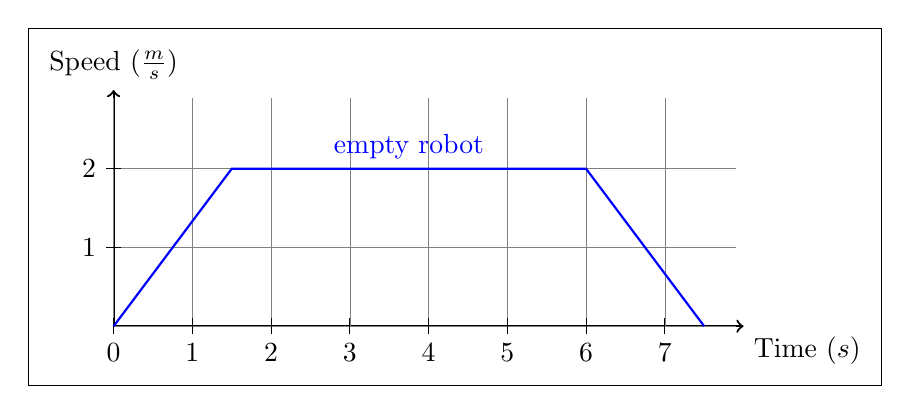
\begin{tikzpicture}[show background rectangle]
    \draw[thick,->] (0,0) -- (0,3) node[above] {Speed ($\frac{m}{s}$)};
    \draw[thick,->] (0,0) -- (8,0) node[below right] {Time ($s$)};
    \draw[very thin, gray] (0,0) grid (7.9,2.9);

    \foreach \x in {0,...,7}
    \draw (\x,0.1) -- (\x,-0.1) node [below] {\x};

    \foreach \y in {1,...,2}
    \draw (0.1,\y) -- (-0.1,\y) node [left] {\y};

    % path
    \draw[thick, blue] (0,0) -- (1.5,2) -- node[above] {empty robot} (6,2) --
    (7.5,0);
\end{tikzpicture}


        \caption{This figure shows the movement of an empty robot in $\Dn$ or
            $\Ds$ direction with moving for 2 parking spaces. The total distance
            traveled is 12 meters, which is exactly the length of 2 parking spaces in
        that direction.}
        \label{fig:manyspaces}
    \end{center}
\end{figure}

\begin{table}
    \begin{center}
        \begin{tabular}{| c | c |}
            \hline
            Action & Time (s)\\
            \hline
            Lift car & 9\\
            Drop car & 3\\
            Accelerate to full speed & 1.5\\
            Deacceleration from full speed to stop & 1.5\\
            Loaded robot moving to adjacent space (N or S) & 7.5\\
            Loaded robot moving to adjacent space (E or W) & 4.5\\
            Empty robot moving to adjacent space (N or S) & 3\\
            Empty robot moving to adjacent space (E or W) & 4.5\\
            \hline
        \end{tabular}
        \TODO{make this table nice}
        \caption{We list different actions and the time they need to complete.}
        \label{tbl:times}
    \end{center}
\end{table}
\subsection{Simplified discrete problem}
\label{sec:discrete problem}
From the~\autoref{tbl:times}, it can be seen that all the times are multiples
of 1.5 seconds. So we can ignore the actual speeds and dimensions. We can just
use multiplies of 1.5 seconds, which we will call timesteps. One timestep is
equal to 1.5 seconds. All the movements take a discrete number of timesteps.
And every movements ends up in the exact center of the parking place.

For the car park, we use graph $\mathcal{G} = (\V,\E)$, where every vertex is a
parking space and every edge $(u,v)$ means that there is no obstacle between
parking spaces~$u$ and~$v$. The parking places can be at most 4-way-connected,
with the connections corresponding to directions in $\D$.

Every parking space has status. We let $K$ be the number of different labels we
want to give to cars. All possible node statuses are described
in~\autoref{tbl:statuses}. We denote the set of all node statuses as~$\W$.

\begin{table}
    \begin{center}
        \begin{tabular}{| c | c |}
            \hline
            Status & Meaning \\
            \hline
            \stat{e} & Parking space is empty.\\
            \stat{r} & There is robot on the parking space.\\
            \stat{i} & There is a car with label $i$ in
            the parking space.\\
            \stat{ri} & There is a car with label $i$ and a robot is under it.\\
            \stat{ir} & There is a robot carrying the car with label $i$.\\
            \stat{lft} & There is a robot in the process of lifting a car.\\
            \stat{drp} & There is a robot in the process of dropping a car.\\
            \hline
        \end{tabular}
        \TODO{make this table nice}
        \caption{We all different possible statuses of parking spaces with
            their descriptions. Note that $\stat{i} \in \{0,\ldots,K-1\}$. So
            when there is a robot carrying car with label 2, the status should
            be \stat{2r}, not \stat{ir}.}
        \label{tbl:statuses}
    \end{center}
\end{table}

When a object moves from node~$u$ to an adjacent node $v$, the initial node
status remains the same for the whole duration of the movement. Meaning that
even though the moving object partly blocks both~$u$ and~$v$, the node statuses
for~$u$ and ~$v$ will still be the old ones, until the moving object reaches the center
of~$v$, at which point node statuses are updated. As an example of this
see~\autoref{fig:movingstatus}.

\begin{figure}[h]
    \begin{center}
        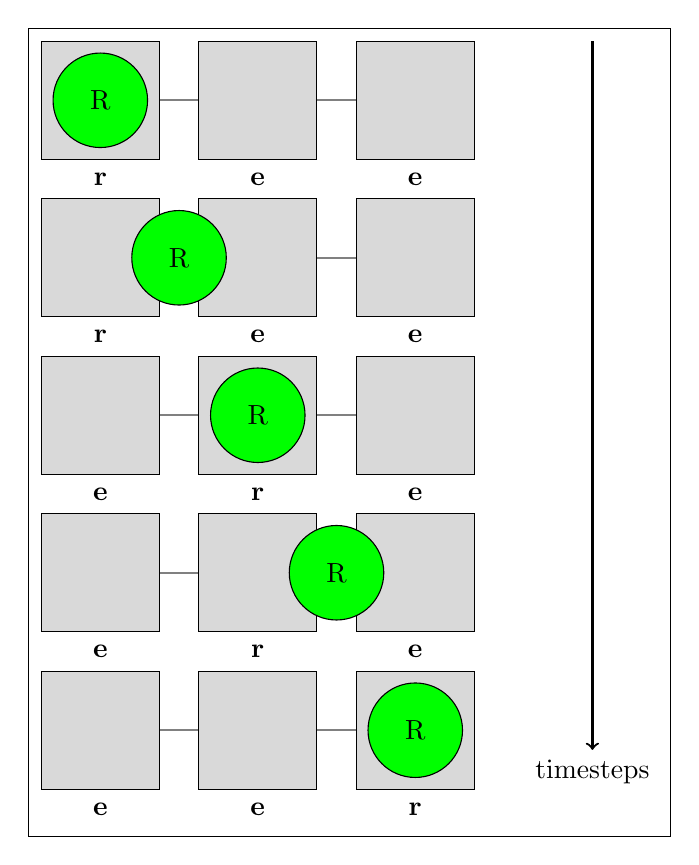
\begin{tikzpicture}[show background rectangle]
% nodes

\foreach \y in {9, 7, 5, 3, 1}
{
    \draw[gray,thick] (0,\y-0.75) -- (5,\y-0.75);
    \draw[fill=gray!30] (0,\y) rectangle (1.5, \y-1.5);
    \draw[fill=gray!30] (2,\y) rectangle (3.5, \y-1.5);
    \draw[fill=gray!30] (4,\y) rectangle (5.5, \y-1.5);
}

\draw[thick, ->] (7,9) -- (7,0) node[below] {timesteps};

\draw[fill=green] (0.75,8.25) node {R} circle (0.6);
\draw[fill=green] (1.75,6.25) node {R} circle (0.6);
\draw[fill=green] (2.75,4.25) node {R} circle (0.6);
\draw[fill=green] (3.75,2.25) node {R} circle (0.6);
\draw[fill=green] (4.75,0.25) node {R} circle (0.6);

\node at (0.75, 7.25) {\stat{r}};
\node at (2.75, 7.25) {\stat{e}};
\node at (4.75, 7.25) {\stat{e}};

\node at (0.75, 5.25) {\stat{r}};
\node at (2.75, 5.25) {\stat{e}};
\node at (4.75, 5.25) {\stat{e}};

\node at (0.75, 3.25) {\stat{e}};
\node at (2.75, 3.25) {\stat{r}};
\node at (4.75, 3.25) {\stat{e}};

\node at (0.75, 1.25) {\stat{e}};
\node at (2.75, 1.25) {\stat{r}};
\node at (4.75, 1.25) {\stat{e}};

\node at (0.75, -0.75) {\stat{e}};
\node at (2.75, -0.75) {\stat{e}};
\node at (4.75, -0.75) {\stat{r}};
\end{tikzpicture}

        \caption{This diagram serves as an illustration for node statuses
            during movement. Each row represents a seperate timestep of the
            same nodes. Gray boxes represent parking spaces and the green
            circle represents a moving robot. Below each parking space is the node
        status.}
        \label{fig:movingstatus}
    \end{center}
\end{figure}

The problem is to find a suitable sequence of actions for robots, to
reconfigure the given initial configuration into the terminal configuration.
Both initial and terminal configurations are given by node statuses for every
vertex.

Sometimes a given initial status with given terminal status is unsolvable no
matter how many timesteps are considered. For a very simple example
see~\autoref{fig:unsolvable}.

\begin{figure}[h]
    \begin{center}
        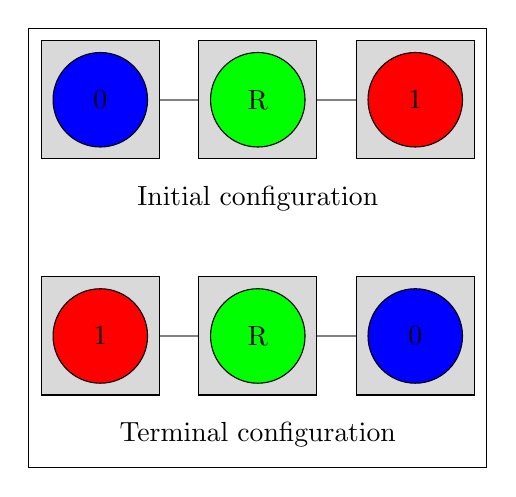
\begin{tikzpicture}[show background rectangle]
% nodes

\foreach \y in {4, 1}
{
    \draw[gray,thick] (0,\y-0.75) -- (5,\y-0.75);
    \draw[fill=gray!30] (0,\y) rectangle (1.5, \y-1.5);
    \draw[fill=gray!30] (2,\y) rectangle (3.5, \y-1.5);
    \draw[fill=gray!30] (4,\y) rectangle (5.5, \y-1.5);
}

\draw[fill=blue] (0.75,3.25) node {0} circle (0.6);
\draw[fill=green] (2.75,3.25) node {R} circle (0.6);
\draw[fill=red] (4.75,3.25) node {1} circle (0.6);

\draw[fill=red] (0.75,0.25) node {1} circle (0.6);
\draw[fill=green] (2.75,0.25) node {R} circle (0.6);
\draw[fill=blue] (4.75,0.25) node {0} circle (0.6);

\node at (2.75, 2) {Initial configuration};
\node at (2.75, -1) {Terminal configuration};

\end{tikzpicture}


        \caption{This figure shows a pair of initial and terminal statuses,
            which cannot be solved. Green robot can move under the cars, but there
            is no way how red car can exchange places with the blue car without
        colliding.}
        \label{fig:unsolvable}
    \end{center}
\end{figure}

%\subsubsection{Canonical form of LP}
\begin{align*}
    &\max c^T \cdot x\\
    &Ax \leq b\\
    &x \geq 0
\end{align*}
\subsubsection{Dual of it}

\begin{align*}
    &\min y^T \cdot b\\
    &y^TA \geq c^T \quad (A^ty \leq c)\\
    &y \geq 0
\end{align*}

\subsubsection{Weak duality theorem}
\begin{theorem}
Primal LP optimum $\leq$ Dual LP optimum
\end{theorem}
\begin{proof}
    For any feasible vector $x$ and for any feasible vector $y$, we show that $c^Tx
    \leq y^Tb$. Because $x$ is feasible we have $Ax \leq b$. Because $y \geq 0$, we
    get that 
\begin{align}
    \label{eq:wdt_1}
    y^TAx \leq y^Tb.
\end{align}
   We also have that $y^TA \geq c^T$. Since $x \geq 0$:
\begin{align}
    \label{eq:wdt_2}
    y^TAx \geq c^Tx.
\end{align}
By combining (\ref{eq:wdt_1}) and (\ref{eq:wdt_2}) we get that $c^Tx \leq y^Tb$. Because
this holds for any feasible $x$ and $y$ we get that $\max c^Tx \leq \min y^Tb$.

\end{proof}
\subsubsection{Strong duality}
\begin{theorem}
    There are a few possibilities.
    \begin{enumerate}
        \item Both primal and dual problems are infeasible.
        \item The primal problem is infeasible and the dual is unbounded.
        \item The primal problem is unbounded and the dual is infeasible.
        \item Both primal and dual problems have feasible solutions and their optimum
            values are equal.
    \end{enumerate}
\end{theorem}

\section{Integer programming model}
\TODO{Write introduction to the model}
\TODO{Should I repeat things mentioned in the introduction? ($\V,\E,\W)$ (sets and
iterators)}
We have to fix the number of timesteps that the model has. We use $\T =
\{0,\ldots,t_{\max}\}$ to denote the set of all timesteps in the model.

Now we define some subsets of node statuses. We start with~$\Wl$, a set of
statuses where robot is under a car and decision to lift it can be made. Second
is almost the opposite set~$\Wd$, which containts all the statuses, where robot
is carrying a car and decision to drop it can be made. Third set is~$\Wm$ and
it consists of statuses, that correspond to moving components. A robot can
move and a robot carrying a car can move.
\begin{align}
    \Wl &= \{\stat{ri} \mid i \in \{0,\ldots,K-1\}\}\\
    \Wd &= \{\stat{ir} \mid i \in \{0,\ldots,K-1\}\}\\
    \Wmc &= \Wd \cup \{\stat{r}\}
\end{align}

\TODO{Explanation of movement}
De-accelerating a moving robot takes 1 timestep. Therefore, the decision to continue
moving in the same direction or to stop has to be made 1 timestep before
arriving at and adjacent node. Since we change the node statuses only when we
arrive at the center of parking place as illustrated
on~\autoref{fig:movingstatus}, the decisions to continue or stop moving are
also made on the same node. The object has not yet arrived at the other node,
so it does not make sense tie to decision with the destination node.

\begin{lemma}
    All feasible solutions to the integer programming model correspond to feasible
    actions of robots and all feasible actions of the robots correspond to
    feasible solutions to the integer programming model.
    \TODO{find good way to write this}
\end{lemma}
\begin{proof}
    This will become clear from the explanations of variables
    in~\autoref{sec:variables} and explanations of constraints
    in~\autoref{sec:constraints}.
\end{proof}
\subsection{Variables}
\label{sec:variables}
The variables for the model are all binary, meaning their allowed values are from the set
$\{0,1\}$. There are three groups of variables:
\begin{enumerate}
    \item node status variables,
    \item edge occupied variables,
    \item decision variables.
\end{enumerate}
For every timestep, there is another layer of the variables. Meaning that if
we have $n$ variables for timestep $0$, and we have $t$ timesteps, then in total
there will be $tn$ variables in the model. In the variable indexing, the
timestep is always the last index.

\subsubsection{Node status variables}
As specified in \autoref{sec:discrete problem}, there are many possible statuses
for parking spots. Node status variables are meant to encode the node status.
There is a variable for every combination of node, status and timestep. To be
more accurate, the group of node status variables is defined as following.
\begin{align}
    &\forall v \in \V \colon \forall w \in \W \colon \forall t \in \T \colon &
    \nstat_{v,w,t}
\end{align}

\subsubsection{Edge occupied variables}
There are variables for each directed edge between parking spots. When a robot
moves from vertex $u$ to vertex $v$ at timestep $t$, the edge variable
$\occu_{(u,v),t}$ is 1 to indicate that the edge is occupied. All edge variables
are defined as:
\begin{align}
    &\forall e \in \E \colon \forall t \in \T \colon & \occu_{e,t}
\end{align}

\subsubsection{Decision variables}
This is the most important group of variables, because they represent the
decisions or actions that the model should find. Before we can give them, we
have to introduce a little function $\dir \colon \E \to \D$. Since we are
operating on not just any graph, but on a grid, we can determine the direction
of the edge and $\dir$ does exactly that. The decision variables are the
following.
\begin{align}
    &\forall e=(u,v) \in \E \colon \forall w \in \Wmc \colon \forall t \in \T \colon
    & \go_{u,w,\dir(e),t}\\
    &\forall e=(u,v) \in \E \colon \forall w \in \Wmc \colon \forall t \in \T
    \colon & \cont_{u,w,\dir(e),t}\\
    &\forall e=(u,v) \in \E \colon \forall w \in \Wmc \colon \forall t \in \T
    \colon & \stp_{u,w,\dir(e),t}\\
    &\forall v \in \V \colon \forall w \in \Wl \colon \forall t \in \T \colon &
    \lift_{v,w,t}\\
    &\forall v \in \V \colon \forall w \in \Wd \colon \forall t \in \T \colon &
    \drop_{v,w,t}
\end{align}
Decision variable is set to 1, if and only if that action is taken at the
specified node, with specified node status, and at specified timestep. For
movement variables: $\go_{v,w,d,t}$, $\cont_{v,w,d,t}$ and $\stp_{v,w,d,t}$
also the direction is specified. Decision variables already have
self-describing names, but to clarify, we explain them one-by-one
in~\autoref{tbl:decvars}.

\begin{table}[h]
    \center
    \begin{tabular}{| c | p{\textwidth - 2.6cm} |}
        \hline
        Variable & Meaning\\
        \hline
        $\go_{v,w,d,t}$ & At timestep $t$ on parking space $v$ with node status
        $w$, a robot starts to accelerate in direction $d$.\\ \hline
        $\cont_{v,w,d,t}$ & At timestep $t$ on parking space $v$ with node status
        $w$ a robot that is about to reach the neighbouring node in direction
        $d$, does not slow down and continues moving in direction $d$.\\ \hline
        $\stp_{v,w,d,t}$ & At timestep $t$ on parking space $v$ with node status
        $w$ a robot that is about to reach the neighbouring node in direction
        $d$, starts to de-accelerate to stop in the neighbouring node.\\ \hline
        $\lift_{v,w,t}$ & At timestep $t$ on parking space $v$ with node status
        $w$ a robot starts to lift a car.\\ \hline
        $\drop_{v,w,t}$ & At timestep $t$ on parking space $v$ with node status
        $w$ a robot starts to drop a car.\\
        \hline
    \end{tabular}
    \TODO{make this table nice}
    \caption{The table explaining the meaning of decision variables.}
    \label{tbl:decvars}
\end{table}

\subsection{Example configurations to illustrate the model}
Before diving into constraints, we give 12 small configurations which will
illustrate the meaning of variables and our assumptions about the integer
programming model.

As a side remark: complexity of the integer programming model is large enough
to not fit into the working memory of humans. Humans can keep about 7 things in
their working memory at once~\cite{magic7}. When developing the model a lot of
time was consumed by manually altering the initial status of the model and then
verifying if the feasible optimal solution to model was indeed a valid sequence
of actions. To cut down the time on manual rewriting of the initial status and
manual verifying of solutions, these illustration configurations were also used
for testing the model during development.

Testing was needed to avoid typos like writing $v$ or even $u$ instead of $v'$.
Also there were some occurrences, where we made wrong assumptions, because there
are so many cases to consider for a simple action.\todo{Write something more
meaningful here.}

Some of these illustrations or tests are meant to be infeasible. Others have
expected outcomes, which are automatically verified . When an specific
objective function is not mentioned, the objective function will be left empty
for that test. By empty objective we means that the objective function is~$\min
0$.

The initial node statuses are fixed for every configuration. To easily display
the initial statuses, we use images that depict the underlying graph of the
problem and the node statuses at timestep 0. In the images, nodes are
represented as circles. They gray lines between nodes show that there is an
edge between those vertices. Inside the circles the upper text shows the node
status and the lower text shows the identifier of the node.
\subsubsection{Collision}
The purpose of this test is to make sure head on collisions are infeasible in
the model.
\testImage{collision}{Initial node statuses for collision test.}
To force a collision, we use the following constraints to fix the values of two decision
variables.
\begin{align}
    \go_{(0,1),\stat{r},\De,0} &= 1\\
    \go_{(1,1),\stat{r},\Dw,0} &= 1
\end{align}
The desired output is infeasibility of the model.
\subsubsection{Collision with same destination}
Next test makes sure two robots cannot move into the same node at the same
time.
\testImage{collision2}{Initial node statuses for collision test with same
destination.}
The following constraints oblige both of the robots to start moving to node $(1,0)$.
\begin{align}
    \go_{(2,0),\stat{r},\Dw,0} &= 1\\
    \go_{(1,1),\stat{r},\Dn,0} &= 1
\end{align}
As with the last test, this model should be infeasible.
\subsubsection{Collision with special}
Last two tests made sure that robots cannot collide, but another test is needed
for robots carrying cars with different labels.
\testImage{collisionspecial}{Initial node statuses for collision test with
loaded robots}
We use the following constraints, which are very similar to constraints used in
the head-on collision test.
\begin{align}
    \go_{(0,1),\stat{0r},\De,0} &= 1\\
    \go_{(1,1),\stat{1r},\Dw,0} &= 1
\end{align}
As with other collision tests, the model should be infeasible.
\subsubsection{Orthogonal collision}
We also have a test for collision with orthogonal directions.
\testImage{collisionorth}{Initial node statuses for collision test with
orthogonal directions}
We use the following constraints to fix the movements.
\begin{align}
    \go_{(1,0),\stat{r},\Dw,0} &= 1\\
    \go_{(1,1),\stat{r},\Dn,0} &= 1
\end{align}
Here robot on $(1,0)$ is moving away from it, and robot on $(1,1)$ is trying to
move into $(1,0)$. This kind of collision is explained
with~\autoref{fig:orthcol}. Because of the collision, the model should be
infeasible.

\begin{figure}[h]
    \begin{center}
        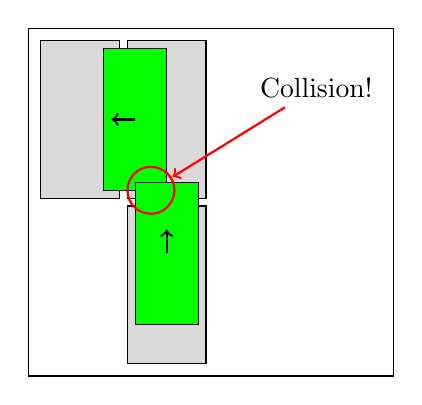
\begin{tikzpicture}[show background rectangle]

\coordinate (A) at (0,2.1);
\coordinate (B) at (1.1,2.1);
\coordinate (C) at (1.1,0);


\foreach \v in {A,B,C}
{
    \draw[fill=gray!30] (\v) + (-0.5,-1) rectangle ++(0.5, 1);
}

\coordinate (D) at (0.7, 2.1);
\coordinate (E) at (1.1, 0.4);

\foreach \v in {D,E}
{
    \draw[fill=green] (\v) + (-0.4,-0.9) rectangle ++(0.4, 0.9);
}

\draw[thick,black,->] (D) -- (0.4,2.1);
\draw[thick,black,->] (E) -- (1.1,0.7);

\node (T) at (3,2.5) {Collision!};
\node[thick, draw, circle, red, scale=1.8] (col) at (0.9,1.2) {};
\draw[thick,red,->] (T) -- (col);

\end{tikzpicture}

        \caption{Green rectangles are robots and gray rectangles are parking
            spaces. One robot is moving away from a parking space and another is
        moving toward it from an orthogonal direction. This causes a collision.}
        \label{fig:orthcol}
    \end{center}
\end{figure}

\subsubsection{Collision with itself}
This is a test to see that edge constraints have the right number of timesteps.
\testImage{collisionself}{Initial node statuses for collision test with
itself.}
\begin{align}
    \go_{(2,0),\stat{r},\Dw,0} &= 1\\
    \go_{(1,0),\stat{r},\De,2} &= 1
\end{align}
When the edges are occupied for longer than actually needed, the model will
become infeasible, because the first movement marks edge $((2,0),(1,0))$ as
occupied, and the second movement marks edge $((1,0),(2,0))$ as occupied. And
they cannot be both occupied at the same time thanks to
constraint~\eqref{eq:antiedges}.

This model should be feasible.
\subsubsection{Simultaneous movement}
With this test, we make sure that robots can move in the same direction side by
side.
\testImage{movetogether}{Initial node statuses for simultaneous movement test.}
Both robots are forced to move at the start.
\begin{align}
    \go_{(1,0),\stat{r},\Dw,0} &= 1\\
    \go_{(2,0),\stat{r},\Dw,0} &= 1
\end{align}
The model should be feasible and a feasible solution is also verified by following
checks, which should hold for all feasible solutions.
\begin{align}
    \nstat_{(0,0), \stat{r}, 2} &\ife 1\\
    \nstat_{(1,0), \stat{r}, 2} &\ife 1\\
    \nstat_{(2,0), \stat{e}, 2} &\ife 1
\end{align}

\subsubsection{Simultaneous movement II}
This is quite similar to last test, but now we have other than empty nodes in
the way and one of the robots is also carrying a car.
\testImage{movetogetherdiff}{Initial node statuses for simultaneous movement
    test with a car on the way and the last robot carrying a car.}
\begin{align}
    \go_{(1,0),\stat{r},\Dw,0} &= 1\\
    \go_{(2,0),\stat{r},\Dw,0} &= 1\\
    \go_{(3,0),\stat{r},\Dw,0} &= 1\\
    \go_{(4,0),\stat{0r},\Dw,0} &= 1
\end{align}
The model should be feasible and optimal solution is verified by following
checks.
\begin{align}
    \nstat_{(1,0), \stat{r1}, 2} &\ife 1\\
    \nstat_{(1,0), \stat{r}, 2} &\ife 1\\
    \nstat_{(2,0), \stat{r0}, 2} &\ife 1\\
    \nstat_{(3,0), \stat{0r}, 3} &\ife 1\\
    \nstat_{(4,0), \stat{e}, 3} &\ife 1
\end{align}

\subsubsection{Invalid simultaneous movement}
This test checks if node statuses are handled correctly when things move
together.
\testImage{movetogetherbad}{Initial node statuses for simultaneous
    movement test with an invalid node status constraint.}
\begin{align}
    \go_{(1,0),\stat{r},\Dw,0} &= 1\\
    \go_{(2,0),\stat{r},\Dw,0} &= 1\\
    \nstat_{(1,0),\stat{r0},2} &= 1
\end{align}
The status of node $(1,0)$ after the movement, at timestep 2 should
be~$\stat{r}$. However, we give a constraint which should make the model
infeasible.
\subsubsection{Lift and move}
This test checks if the model can find a correct solution to a simple problem.
\testImage{liftandmove}{Initial node statuses for the lift and move test.}
This time instead of adding constraints to force some actions, we define the
objective function.
\begin{align}
    \min \sum_{t \in \T} -\nstat_{(0,0), \stat{r0}, t}
\end{align}
Correct solution would be for the robot to move into the middle node $(1,0)$,
lift the car from there and carry it to $(0,0)$ and finally drop it there. The
solution is checked against the following conditions.
\begin{align}
    \nstat_{(0,0), \stat{e}, 2} &\ife 1\\
    \nstat_{(1,0), \stat{r0}, 2} &\ife 1\\
    \nstat_{(2,0), \stat{0}, 2} &\ife 1\\
    \nstat_{(1,0), \stat{0r}, 8} &\ife 1\\
    \nstat_{(0,0), \stat{0r}, 11} &\ife 1\\
    \nstat_{(0,0), \stat{r0}, 13} &\ife 1
\end{align}
These conditions just make sure that node statuses at various timesteps are
correct.
\subsubsection{Lift and move forced}
This test is almost the same as previous, but now the decisions are forced with
the following constraints.
\testImage{liftandmoveforced}{Initial node statuses for the forced lift and move test.}
\begin{align}
    \go_{(2,0),\stat{r},\Dw,0} &= 1\\
    \lift_{(1,0),\stat{r1},2} &= 1\\
    \go_{(1,0),\stat{1r},\Dw,8} &= 1\\
    \nstat_{(0,0),\stat{e},8} &= 1
\end{align}
The objective is now to issue as many lifts at node $(0,0)$ for car with label 1
as possible.
\begin{align}
    \min \sum_{t \in \T} -\lift_{(0,0), \stat{r1}, t}
\end{align}
The solution is checked against these conditions.
\begin{align}
    \nstat_{(0,0), \stat{e}, 2} &\ife 1\\
    \nstat_{(1,0), \stat{r1}, 2} &\ife 1\\
    \nstat_{(2,0), \stat{0}, 2} &\ife 1\\
    \nstat_{(1,0), \stat{1r}, 8} &\ife 1\\
    \nstat_{(0,0), \stat{1r}, 11} &\ife 1
\end{align}
When the previous test failed, the model did something else to obtain a better
objective value. This test was added to see, if a legal sequence of decisions
was indeed feasible during the development of constraints.
\subsubsection{Persistence, no robots}
This test is to make sure that node statuses stay the same when there are no
robots.
\testImage{persistence}{Initial node statuses for the persistence test.}
We also add one odd constraint.
\begin{align}
    \nstat_{(0,0),\stat{r},20} &= 1
\end{align}
And the objective function used is different to encourage occupying edges and
appearance of robots.
\begin{align}
    \min \sum_{t \in \T}\left( -4\nstat_{(0,0), \stat{r}, t}
    -4\nstat_{(1,0),\stat{r},t} -\sum_{e \in \E} \occu_{e,t} \right)
\end{align}
Of course node statuses should not change by themselves, and the model should be
infeasible.

\subsubsection{Continue together}
This tests makes sure that robots can continue moving in one direction, even
when moving together. Actually it tests both a single robot continuing and at
the same time also 2 robots continuing together.
\testImage{largetest}{Initial node statuses for the continue test.}
The objective is for robots to go to the right side.
\begin{align}
    \min \sum_{t \in \T} -\nstat_{(3,0), \stat{r}, t} -\nstat_{(3,1),\stat{r},t} -\nstat_{(2,1),\stat{r},t}
\end{align}
The model should be feasible and the optimal solution is verified by hand.

\subsection{Constraints}
\label{sec:constraints}
\subsubsection{Helper functions and notation for constraints}
\label{sec:helpers}
The first helper function used is $\edg \colon \V \times \D \to \V$. Let
$\edg(v,d)$ denote the node that is in the direction $d$ from node $v$.

For directions we use $d + 1$ to denote the next direction from direction $d$ in
clockwise manner. Logically $d - 1$ is used to mark the next direction from $d$
in counterclockwise manner. For an example: $\Dn + 1 = \De$.

Some decisions take a specified amount of time. We want to disallow making such
decisions, which lead to actions that cannot be completed in the time frame of
the model. For this purpose we want to split $\T$ into two disjoint subsets.
Let $\T_i = \{ t | (t+i) \in \T\}$ and $\Tn_i = \T \setminus \T_i$.

The decisions to stop moving or continue moving are mostly used together.
Either one of those implies that node status is about to change. For that
reason we use an abbreviation $\contOrStop_{u,w,d,t} = \cont_{u,w,d,t} +
\stp_{u,w,d,t}$.
\TODO{Add more meaningful stuff here}
\subsubsection{Simple constraints}
\label{sec:simple}
First constraint is to make sure that at every timestep each node has exactly
one status variable set.
\begin{align}
    &\forall v \in \V \colon \forall t \in \T \colon & \sum_{w \in \W}
    \nstat_{v,w,t} = 1
\end{align}
When a directed edge is used, its opposite cannot be used at the same time.
\begin{align}
    \label{eq:antiedges}
    &\forall (u,v) \in \E \colon \forall t \in \T \colon & \occu_{(u,v),t} +
    \occu_{(v,u),t} \leq 1
\end{align}
No more than one moving thing can arrive at the same node at the same time.
\begin{align}
    &\forall v \in \V \colon \forall t \in \T \colon & \sum_{u \in \N(v)}
    \occu_{(u,v),t} \leq 1
\end{align}
We also want to forbid movements in the orthogonal directions.
\begin{equation}
    \begin{split}
        \forall v \in \V \colon \forall d \in \D \colon \forall t \in \T \colon
        \quad & \occu_{(\edg(v,d),v),t} \\ + \occu_{(v,\edg(v,d-1)),t} + &
        \occu_{(v,\edg(v,d+1)),t} \leq 1
    \end{split}
\end{equation}
Note that there are vertices such that they do not have an edge between them, or
they do not even have a neighbour in some directions. When that happens, the
invalid $\occu_{e,t}$ variables are not added to the sum.
Also it does not make sense to allow more than 1 decision at the same time, at
the same location.
\begin{equation}
    \begin{split}
        \forall v \in \V \colon \forall t \in \T \colon \quad & \sum_{d \in \D,
        w \in \Wmc}(\go_{v,w,d,t} + \stp_{v,w,d,t} + \cont_{v,w,d,t}) \\ + &
        \sum_{w \in \Wl} \lift_{v,w,t} + \sum_{w \in \Wd} \drop_{v,w,t} \leq 1
    \end{split}
\end{equation}

\subsubsection{Lifting and dropping constraints}
These constraints describe the lifting and dropping of cars. In fact they are
quite similar, they indeed are opposite actions. We will start with lifting
constraints. Instead of using $\T$, like we did in~\autoref{sec:simple}, we use
$\T_6$, because lifting takes 6 timesteps. First constraint type is to make sure
that the node status is correct, when a decision to lift is made.
\begin{align}
    &\forall v \in \V \colon \forall w \in \Wl \colon \forall t \in \T_6 \colon
    &\lift_{v,w,t} - \nstat_{v,w,t} \leq 0
\end{align}
While the lifting is in progress, we want the node status be fixed to
$\stat{lft}$.
\begin{align}
    &\forall v \in \V \colon \forall w \in \Wl \colon \forall t \in \T_6 \colon
    \forall i \in \{1,\ldots,5\} \colon &\lift_{v,w,t} -
    \nstat_{v,\stat{lft},t+i} \leq 0
\end{align}
And at the end of lifting, the node status should correspond to the lifted
thing. For that we have a simple helper function $f \colon \Wl \to \Wd$. It is
defined as: $f(\stat{rc}) = \stat{cr}$ and $\forall j \colon
f(\stat{rsc}_j) = \stat{scr}_j$. In words, the function $f$ determines the node
status after lifting. By using $f$ we can now give the set of constraints.
\begin{align}
    &\forall v \in \V \colon \forall w \in \Wl \colon \forall t \in \T_6 \colon
    &\lift_{v,w,t} - \nstat_{v,f(w),t+6} \leq 0
\end{align}
If the lifting cannot be completed, we just make sure that the decision is
never made.
\begin{align}
    &\forall v \in \V \colon \forall w \in \Wl \colon \forall t \in \Tn_6
    \colon &\lift_{v,w,t} = 0
\end{align}

For dropping we have almost the same constraints. First make sure that the node
status is correct, when decision is made.
\begin{align}
    &\forall v \in \V \colon \forall w \in \Wd \colon \forall t \in \T_2 \colon
    &\drop_{v,w,t} - \nstat_{v,w,t} \leq 0
\end{align}
Dropping takes less time than lifting, therefore the constraints for
intermediate node state are simpler than for lifting.
\begin{align}
    &\forall v \in \V \colon \forall w \in \Wd \colon \forall t \in \T_2 \colon
    &\drop_{v,w,t} - \nstat_{v,\stat{drp},t+1} \leq 0
\end{align}
To get the correct node status at the end of the drop, we can use the inverse
of the previous helper function $f$.
\begin{align}
    &\forall v \in \V \colon \forall w \in \Wd \colon \forall t \in \T_2 \colon
    &\drop_{v,w,t} - \nstat_{v,f^{-1}(w),t+2} \leq 0
\end{align}
As with lifting, if dropping action cannot be completed in the time frame of
the model, disable the decision.
\begin{align}
    &\forall v \in \V \colon \forall w \in \Wd \colon \forall t \in \Tn_2
    \colon &\drop_{v,w,t} = 0
\end{align}

\subsubsection{Moving constraints}
Depending on the direction and whether the robot is carrying a car, the
movement takes different number of timesteps. We introduce a new function $g
\colon \W \times \D \to \mathcal{N}$. Function $g(w,d)$ returns the number of
timesteps the movement of $w$ takes in direction $d$. 

Now movement constraints are tricky and constructing them needs some
abbreviations. The constraints in this section are for all combinations of $u
\in \V$, $w \in \Wmc$, $d \in \D$ and $t \in \T$.
\TODO{Fix this paragraph}

Now let $\td = g(w,d)$, and $\td' = \td-1$. When movement starts at time $t$,
the node status will change at time $t+\td$, and at time $t+\td'$ a decision
has to be made to continue moving in the same direction or stop. Let $v =
\edg(u,d)$ be the destination node and $e = (u,v)$ the edge that is used for
movement. Later we also need $u' = \edg(u,d+2)$\footnote{$d+2$ means the
opposite direction from $d$}, which is the node before $u$ and $v' =
\edg(v,d)$, which is the node after $v$. Also we need the set of node statuses
where the moving component $w$ could came from.
\begin{align}
    \uw = \{w_m \mid w_m \in \Wm \wedge \getMC(w_m) = w\}
\end{align}
When $e \notin \E$ we skip the constraints, because we do not have movement
variables for such a combination of starting vertex $u$ and direction $d$. Also
when $t+\td' \notin \T$ we disable the start of movement, because it cannot
continue.
\begin{align}
    &\IF{t+\td' \notin \T} &\go_{u,w,d,t} = 0
\end{align}
In addition to disabling go, we skip the rest of the constraints.

As with other decisions the first group of constraints make sure that node
status is correct at the time of the decision. In our case it has to be one of
the possible node statuses in $\uw$.
\begin{align}
    & \go_{u,w,d,t} - \sum_{w_u \in \uw} \nstat_{u,w_u,t} \leq 0
\end{align}
If we have the edge $(u',u) \in \E$, that means that an already moving object
could continue moving from $u'$ and is in other ways equivalent to a moving
object, that start accelerating from $u$. So we define an abbreviation.
\begin{align*}
    \goOrCont = \begin{cases}
        \go_{u,w,d,t} \IFc (u',u) \notin \E\\
        \go_{u,w,d,t} + \cont_{u',w,d,t} \IFc (u',u) \in \E
    \end{cases}
\end{align*}
and a constraint to make sure that those things do not happen at the same time.
\begin{align}
    \goOrCont \leq 1
\end{align}
When there is movement, it has to be continued or stopped.
\begin{align}
    \label{eq:goImpcont}
    \goOrCont - \stp_{u,w,d,t+\td'} - \cont_{u,w,d,t+\td'} = 0
\end{align}
Now again we have to check if movement can actually be completed. Earlier we
checked if $t+\td' \notin \T$ and skipped the rest of the constraints. However
now we check for $t+\td \not \T$. When that happens, we again disable the
movement.
\begin{align}
    &\IF{t+\td' \notin \T} &\go_{u,w,d,t} = 0
\end{align}
And skip the rest of the constraints. At first this seems redundant, but we
need to do it like this, because otherwise constraint~\eqref{eq:goImpcont} would
not exist for $\cont$ and $\stp$ variables at the last timestep and no
constraint would stop them form obtaining value 1.

For the duration of movement the edge $e$ must be occupied and the node status
should remain same. However from $w$, we do not know the actual status of $u$,
therefore we have to go through all possibilities.
\begin{align}
    \forall i \in \{0,\ldots,\td'\}\colon \  \goOrCont - \occu_{e,t+i} &\leq 0\\
    \forall i \in \{1,\ldots,\td'\}\colon \forall w_u \in \uw\colon \ \goOrCont
    + \nstat_{u,w_u,t} - \nstat_{u,w_u,t+i} &\leq 1
\end{align}
There is a simple check: if edge $(v,v') \notin \E$, we can disable continue at
$u$, because after reaching $v$ the robot cannot continue to $v'$. Also when
$t$ is so small, that a previous continue or go decision could not be made, we
disable both the stop and continue at time $t$.
\begin{align}
    &\IF{(v,v') \notin \E} &\cont_{u,w,d,t+\td'} = 0\\
    &\IF{t < \td'} &\cont_{u,w,d,t} = 0\\
    &\IF{t < \td'} &\stp_{u,w,d,t} = 0
\end{align}
\TODO{Maybe a figure showing robots moving together.}
Specifying node statuses for $u$ and $v$ after the movement would be simpler,
if things could not move together. However robots can move side-by-side, at the
same direction. For that reason we need to define additional set of node
statuses. And corresponding variables. When the robot moves away from $u$,
another thing can at the same time move into $u$. For that purpose, we define
the set of statuses, that can move behind $w$ as $\B$. At the same time another
moving object can disappear from $v$. Let $\A$ denote the set of things that
can move ahead of $w$.
\begin{align}
    &\B = \begin{cases}
        \Wmc \IFc w = \stat{r}\\
        \Wd \IFc w \neq \stat{r}
    \end{cases}
    &\A = \begin{cases}
        \{\stat{r}\} \IFc w = \stat{r}\\
        \Wmc \IFc w \neq \stat{r}
    \end{cases}
\end{align}
Now we construct the set of variables, which imply that some additional object
is coming into $u$.
\begin{align}
    \um = \begin{cases}
        0 \IFc (u',u) \notin \E\\
        \sum_{w_{u'} \in \B} \cont_{u',w_{u'},d,t+\td'} +
        \stp_{u',w_{u'},d,t+\td'} \IFc (u',u) \in \E
    \end{cases}
\end{align}
Now we can give the general constraint, which says something about $u$ status
at the end of movement. When $w$ moves away from $u$, it's status should be the
beginning status minus the $w$, or something else must have come into $u$.
\begin{align}
    \stp_{u,w,d,t+\td'} + \cont_{u,w,d,t+\td'} - \ul -\um \leq 0
\end{align}
The last constraint was a general one, that did not exactly specify the status
of $u$ after movement. To actually specify the status of $u$ after movement, we
need to go over all possible $w_u \in \uw$. When $u$ status is about to change
by continuing or stopping, and the $u$ status was $w_u$, the new status should
be $\remMC(w_u)$\footnote{$w_u$ without the moveable component} or something
else moved at the same time into $u$.
\begin{align}
    \begin{split}
        \forall w_u \in \uw\colon\quad &\stp_{u,w,d,t+\td'} + \cont_{u,w,d,t+\td'}
        - \um\\ &+ \nstat{u,w_u,t+\td'} -\nstat_{u,\remMC(w_u),t+\td'} \leq 1
    \end{split}
\end{align}
When there is the edge $(u\,u) \in \E$ only then the following group of
constraints is added. These make sure that if $w_b \in \B$ moved from $u'$ to $u$
the new status of $u$ will be what would be left in $u$ plus the thing that
moved in. There is one catch, what is left into $u$ is car and a robot carrying
a car cannot come to $u$.
\begin{align}
    \begin{split}
        \forall w_u \in \uw\colon &\forall w_b \in \B\colon \quad
        \cont_{u',w_b,d,t+\td'} + \stp_{u',w_b,d,t+\td'}\\
        &+\nstat_{u,w_u,t+\td'}
        -\nstat_{u,\addMC(\remMC(w_u), w_b),t+\td} \leq 1
    \end{split}
\end{align}

Now we want to say something about $v$ status at the end of movement. For that
we use construct the set of statuses that are possible for $v$ after $w$ has
moved into it. It turns out that the set is exactly $\uw$. Movement implies
that at the end $v$ has one of statuses in $\uw$.
\begin{align}
    \begin{split}
        \cont_{u,w,d,t+\td'} + \stp_{u,w,d,t+\td'} -\sum_{w_v \in \uw}
        \nstat_{v,w_v,t+\td} \leq 0
    \end{split}
\end{align}
Similarly to $\um$ we construct the set of variables, which imply that something is
moving away from $v$.
\begin{align}
    \vl = \begin{cases}
        0 \IFc (v,v') \notin \E\\
        \sum_{w_v \in \A} \cont_{v,w_v,d,t+\td'} +
        \stp_{v,w_v,d,t+\td'} \IFc (v,v') \in \E
    \end{cases}
\end{align}
Now we loop over all possible status that $v$ could have at the end of the
movement and specify the actual status. If the end status of $v$ is $w_v$ then
status of $v$ was $\remMC(w_v)$ or something moved away from $v$.
\begin{align}
    \begin{split}
        \forall w_v \in \uw\colon \quad
        \cont_{u,w,d,t+\td'} + \stp_{u,w,d,t+\td'}
        &-\nstat_{v,\remMC(w_v),t+\td'}\\
        &+\nstat_{v,w_v,t+\td} -\vl \leq 1
    \end{split}
\end{align}
\subsubsection{Node status constraints}
Purpose of node status constraints is to make sure that node statuses remain
unchanged when no movement occurs. As with moving constraints, we declare that
the remainder of the section is applied to all possible combinations of $u \in
\V$, $w \in \W$ and $t \in \T_1$.

The basic idea is to list all variables that could change the status of $u$
between timesteps $t$ and $t+1$. We define a lot of sets and then finally use
the union of them. First are the lift and drop variables for the
current timestep~$t$.
\begin{align}
    &\A_{\mathrm{lift}} = \begin{cases}
        \{\lift_{u,w,t}\} \IFc w \in \Wl\\
        \emptyset \IFc w \notin \Wl
    \end{cases}
    &\A_{\mathrm{drop}} = \begin{cases}
        \{\drop_{u,w,t}\} \IFc w \in \Wd\\
        \emptyset \IFc w \notin \Wd
    \end{cases}
\end{align}
Next are the lift and drop variables that happened in the past.
\begin{align}
    \B_{\mathrm{lift}} &= \begin{cases}
        \{\lift_{u,w_l,t-5} \mid w_l \in \Wl\} \IFc w = \stat{lft} \wedge
        t \in \T_{-5}\\
        \emptyset \IFco
    \end{cases}\\
    \B_{\mathrm{drop}} &= \begin{cases}
        \{\drop_{u,w_d,t-1} \mid w_d \in \Wd\} \IFc w = \stat{drp} \wedge
        t \in \T_{-1}\\
        \emptyset \IFco
    \end{cases}
\end{align}
Now there are the movement variables. Only continue and stop variables actually
correspond to immediate node status changes.
\todo{$w_m$ is wrong here}
\begin{align}
    \A_{\mathrm{move}} &= \begin{cases}
        \{\contOrStop_{u,w_m,d,t} \mid w_m \in \Wm \wedge \getMC(w_m) = w\} \IFc
        (\edg(u,d),u) \in \E\\
        \emptyset \IFco
    \end{cases}\\
    \B_{\mathrm{move}} &= \begin{cases}
        \{\contOrStop_{v,w_m,d+2,t} \mid w_m \in \Wm \wedge \getMC(w_m) = w\} \IFc
        (u,\edg(u,d)) \in \E\\
        \emptyset \IFco
    \end{cases}
\end{align}
Now that we have defined all the subpart we join them together.
\begin{align}
    \B &= \B_{\mathrm{lift}} \cup \B_{\mathrm{drop}} \cup \B_{\mathrm{move}} \\
    \A &= \A_{\mathrm{lift}} \cup \A_{\mathrm{drop}} \cup \A_{\mathrm{move}}
\end{align}
Now we can finally give the constraints. The following constraints say that
only one action from the set of node status changing actions can happen at
once. There are two sets, because with simultaneous movement, it can happen
that one action is for moving away and another for moving into~$u$.
\todo{Write explanations}
\begin{align}
    \sum_{v \in \B} v \leq 1\\
    \sum_{v \in \A} v \leq 1
\end{align}
When node status for~$u$ is~$w$, the node status has to remain same or some
kind of action must have changed it.
\begin{align}
    \nstat_{u,w,t} - \nstat_{u,w,t+1} -\sum_{v \in \B} v -\sum_{v \in \A} v
    \leq 0
\end{align}
If node status in the future is~$w$ and something came into the node, another
thing must have left the node.
\begin{align}
    \nstat_{u,w,t+1} +\sum_{v \in \B} v -\sum_{v \in \A} v
    \leq 1
\end{align}
\subsubsection{Edge occupied constraints}
These constrains are to make sure, that when no movement is using an edge the
edge occupied variable will be 0. Constraints in this section are applied for
all combinations of $e=(u,v) \in \E$ and $t \in \T$.
Let $d$ denote the direction of edge $e$. First we collect all variables
which imply that edge is occupied.
\begin{align}
    \A = \sum_{w \in \Wmc,\td \in \{0,\ldots,\getMT(d,w)\}, t+\td \in T}
    \stp_{u,w,d,t+\td} + \cont_{u,w,d,t+\td}
\end{align}
It is quite natural, that only of two of them can actually be 1. If we did not
allow object to move together then only one of the variables could be 1. The
reasoning is that at time $t$ an object moves away from $u$ but at the end of
the movement ($t+\td-1$) another object which entered $u$ at time $t$ could
also leave it.
\todo{Bad explanation}
\begin{align}
    \A \leq 2
\end{align}
We would want an equality constraint $\occu_{e,t} - \A = 0$ which would tell
us that, edge is occupied when movement implied it, and movement occurs, when
edge is occupied. However, $\A$ is not binary as $\occu_{e,t}$ and can also be
2, therefore we need to simulate the equality constraint with two inequality
constraints.
\begin{align}
    \occu_{e,t} - \A &\leq 0\\
    2\occu_{e,t} - \A &\geq 0
\end{align}
\subsection{Initial status and objective}
Initial status will be fixed by adding constraints. Let the initial
status of node $v$ be $v_i$, then we can add constraints to fix node status
variables at the first timestep.
\begin{align}
    &\forall v \in \V\colon &\nstat_{v,v_i,0} = 1
\end{align}
Let $v_e$ denote the end status of node $v$. There are different ways to make
the model find a solution. One way is to add constraints for the last timestep.
\begin{align}
    &\forall v \in \V\colon &\nstat_{v,v_e,t_{\max}} = 1
\end{align}
We still have not defined the objective function to the model. We can
define the objective function in a way that we do not need the constraints for
the end status.
\begin{align}
    \min \sum_{v \in \V,t \in \T} -\nstat_{v,v_e,t}
\end{align}
This objective means that for every node~$v$, we want the status be~$v_e$ for
as long as possible or in other words, as soon as possible.

Other possible objective functions can be considered. Maybe it does not make
sense to add all node statuses to objective. If we ignore the empty nodes, we
can decrease the number of variables in the objective.
\begin{align}
    \label{eq:timeobj}
    \min \sum_{v \in \V,t \in \T,v_e \neq \stat{e}} -\nstat_{v,v_e,t}
\end{align}
\TODO{Show an example why this is bad - rnd-03x03-a, with 30 timesteps}

\TODO{think this over, maybe give on concrete objective here, and discuss about
others somewhere else.}
Sometimes the optimal solution consist of one robot waiting for other to move
out of way. Instead of standing still, the waiting robot moves back and forth.
This is undesired behaviour of the model, because it wastes energy. Therefore
another possible objective function would be to use the end status constraints
and then minimize energy used.
\begin{align}
    \begin{split}
        \label{eq:energyobj}
        \min \sum_{v \in \V,w \in \Wmc,t \in \T,d \in \D, (v,\edg(v,d)) \in \E}
        &C_{1,w} \go_{v,w,d,t} + C_{2,w} \cont_{v,w,d,t} + C_{3,w} \stp_{v,w,d,t}\\
        +\sum_{v \in \V, w \in \Wl,t \in \T} &D_{1,w} \lift_{v,w,t}
        +\sum_{v \in \V, w \in \Wd,t \in \T} D_{2,w} \drop_{v,w,t}
    \end{split}
\end{align}
\TODO{do we want something like that?}
Here $C$ is $(3 \times |\Wmc|)$-dimensional matrix that contains the amount of
energy used by the movement.
This would give optimal solutions energy-wise,
but we are more concerned about time. Minimizing the energy in the case when
there are multiple robots, would lead to only one robot working at the same
time, because working in parallel might take more energy. Therefore a combination of
both~\eqref{eq:energyobj} and \eqref{eq:timeobj} would be the better.

\subsection{Size of the model}

\section{Implementation}
For implementing the model, there were at least two major decisions to be made.
\begin{itemize}
    \item Which optimization software to use?
    \item What programming language to use for generating the model?
\end{itemize}
The author had previous experience with a commercial grade optimization solver
called Gurobi~\cite{gurobi}. It is advertised as a state-of-the-art
mathematical programming solver and it has a free, full-featured academic
license.

Other capable solvers for integer programming models according
to~\cite{meindl2012analysis,mittleman} are CPLEX~\cite{cplex} and XPRESS~\cite{xpress}.
However, they are also both commercial like Gurobi and Gurobi was to easiest to
get an academic licence for.

Gurobi has bindings for several languages. The ones considered were C++ and
Python. It is well known that Python as an interpreted language has a constant
runtime overhead. However, C++ has lots of unwanted complexity. The author
chose to use Python, because generating the integer programming model would
only take a fraction of the time to actually solve it. And the model solving
is not hindered by the runtime system of Python. Because there exist lots of
code that still uses version 2.X of Python, it should be explicitly
mentioned that Python 3.X was used in thesis. To be precise, the exact version
was Python 3.5.1.
\subsection{PANDA}
Programmers are used to thinking in terms of if-clauses. However, in an integer
programming model there are no ifs. At first it was hard to come up with
constraints. We knew which variables were involved and what values were legal,
but writing them as a constraint was still unintuitive. Finding the right
constraint when there were five or more variables proved hard to do by
hand. Fortunately there is a tool called PANDA~\cite{panda} to help with
finding constraints.

PANDA is short for Parallel AdjaceNcy Decomposition Algorithm and its internal
algorithm is more or less the same as Fourier-Motzkin elimination algorithm,
which is taught at the University of Tartu in the course MTAT.05.120
``Combinatorial Optimization''.

PANDA takes an input file, which list the variables and feasible values of the
variables. Then it processes this list of feasible values and outputs a
complete system of equalities and inequalities that hold between the variables.
As an example here is the contents of an valid input file.
\begin{verbatim}
Names:
occu incoming

Vertices:
0 0
1 1
1 2
\end{verbatim}
And the corresponding output by PANDA is:
\begin{verbatim}
PANDA -- facet enumeration with double description
Inequalities:
-2occu +incoming <= 0
occu -incoming <= 0
occu <= 1
\end{verbatim}

Writing input files for PANDA is a little tedious, because you have to list all
the feasible assignments of values to variables. We wrote little programs with
regular if-clauses to generate input files for PANDA. PANDA outputs lots of
inequalities, but some of them are trivial and already covered by other
constraints in the model. Therefore, human judgement was still needed to see
which inequalities and equalities added something valuable to the integer
programming model.
\subsection{Graphical visualization}
For testing the model and seeing the solutions found, we needed some kind of
feedback. At first we had a textual output of the node status and decision
variables for each timestep, it is depicted on~\autoref{fig:nogui}.

\begin{figure}[h]
    \begin{center}
	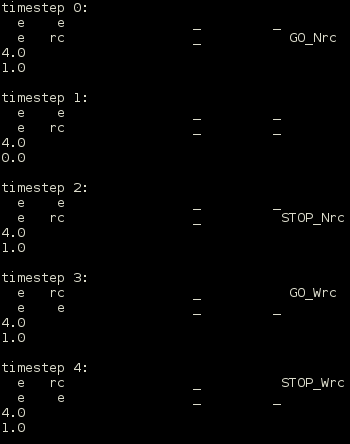
\includegraphics[scale=0.7]{fig/nogui.png}
        \caption{Early textual output of variables. On the left are the node
            statuses for a 2x2 grid and on the right are the decision variables.
        Note that the variables were different then.}
        \label{fig:nogui}
    \end{center}
\end{figure}

However, when the time came to find out, if edge occupied variables had
reasonable values in the solution, the textual output was not good enough to
display the directed edges well. Instead of improving the textual output, we
chose to implement the visualization of solutions graphically.

Because the visualization was used mostly for debugging purposes, there was not
a lot of effort and time put into writing it. To minimize the effort we wrote
the graphical visualization using the de-facto standard Python graphical user
interface package TkInter~\cite{tkinter}. The graphical visualization shows the
underlying graph of the problem one timestep at a time. There are keybindings
to increase and decrease the visible timestep. For a given timestep, the
occupied edges are highlighted. At each vertex, the node status is displayed
and if one of the decision variables was set to 1, the decision is also displayed
inside the vertex. A screenshot of the visualization graphical interface is
on~\autoref{fig:gui}.

\begin{figure}[h]
    \begin{center}
	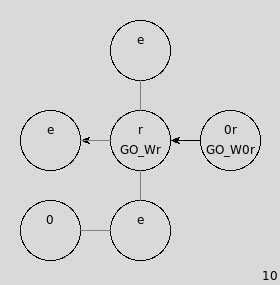
\includegraphics[scale=0.6]{fig/app/ex10.png}
        \caption{Screenshot of the graphical visualization. Circles are the
            nodes, gray lines between them show edges. Black arrows show
            occupied edges. Inside the nodes, the upper text displays the node
            status and the lower text the current decision. In the lower right
        corner is a number, which show the current timestep. }
        \label{fig:gui}
    \end{center}
\end{figure}

\subsection{Irreducible inconsistent subsystem}
In the development phase errors were made. Sometimes a feasible movement were
not feasible in the integer programming model. This would mean that all the
constraints would need to be carefully verified again. Luckily, Gurobi can
calculate an irreducible inconsistent subsystem of an infeasible model.
Inconsistent subsystem of an integer program is a subset of constraints, that
are inconsistent. Irreducible inconsistent subsystem is a minimal
inconsistent subsystem. Basically we can ask Gurobi to find out which set of
constraints make the model infeasible. After we get such a set, we only have to
recheck the constraints that are in the irreducible inconsistent subsystem.

As an example here is the irreducible inconsistent subsystem given by Gurobi
for the orthogonal collision illustration in~\autoref{sec:orthcoltest}.
\begin{verbatim}
Minimize
 
Subject To
 R432: occu(((1,0),(0,0)),0) + occu(((1,0),(2,0)),0)
   + occu(((1,1),(1,0)),0) <= 1
 R5655: - occu(((1,0),(0,0)),0) + go((1,0),'r','W',0)
   + cont((2,0),'r','W',0) <= 0
 R5792: - occu(((1,1),(1,0)),0) + go((1,1),'r','N',0) <= 0
 R6328: cont((2,0),'r','W',0) = 0
 R8494: go((1,0),'r','W',0) = 1
 R8495: go((1,1),'r','N',0) = 1
Bounds
 occu(((1,0),(0,0)),0) free
 occu(((1,1),(1,0)),0) free
 go((1,0),'r','W',0) free
 go((1,1),'r','N',0) free
 cont((2,0),'r','W',0) free
Generals
 occu(((1,0),(0,0)),0) occu(((1,0),(2,0)),0) occu(((1,1),(1,0)),0)
 go((1,0),'r','W',0) go((1,1),'r','N',0) cont((2,0),'r','W',0)
End
\end{verbatim}
\subsection{Tuning Gurobi parameters}
Gurobi might be the best mixed integer program solver around, but as the
problems are NP-complete, it still takes a long time to find the optimal
solution. Gurobi has a lot of parameters~\cite{gurobiparams} that can be
altered, which affect the total runtime. Finding a good set of parameters to
tune is a tedious task, therefore Gurobi comes with an automatic tuning tool.
The tuning tool has an API, but the easiest way is to run it from command line
as a separate tool called \textit{grbtune}.

The tuning tool will take as input integer programming models and then optimize
them many times in a row to establish a baseline performance. After the
baseline is established it will try different set of parameters and it then
outputs those sets that improved on the baseline performance.

Different objective functions leaded to different parameters. When we used
objective function~\eqref{eq:timeobj} with the terminal configuration fixed
with constraints~\eqref{eq:termcont}, \textit{grbtune} reported the following
set of parameters.
\begin{itemize}
    \item MIPFocus = 2
    \item Presolve = 2
    \item PrePasses = 3
    \item Cuts = 0
\end{itemize}

However, when I switched to objective function~\eqref{eq:objective} and
without the terminal configuration constraints, the only parameter that Gurobi
tuning tool found was:
\begin{itemize}
    \item AggFill = 5
\end{itemize}

Now we briefly explain the settings. In the first case MIPFocus is used to
controls the focus of MIP solver. Focus 2 means to work on the best bound.
Presolve controls the aggressiveness of pre-solving the model. Value of 2 means
that pre-solving is aggressive. PrePasses is used to limit the number of
pre-solving passes. Cuts = 0 turns off all cut generations. AggFill controls
the fill level in pre-solve aggregations, with larger values generally lead to
more presolved rows and columns, but at the same time leave more non-zeros in
the constraint matrix~\cite{gurobiparams}.

\section{Comparison}
\TODO{introduction}


\begin{table}
    \begin{center}
        \begin{tabular}{|c|c|c|c|c|c|c|}
            \hline
            Instance & tlimit & $\tm$ & Cap & C & Cap & C\\
            \hline
            marsi3a-1011 & 1h & 50 & 64.53 & 0 & 96.23 & 2\\
            marsi3a-1111 & 1h & 70 & 97.38 & 2 & 95.74 & 3\\
            marsi3a-2111 & 1h & 50 & 92.70 & 1 & 95.83 & 3\\
            marsi3b-1011 & 1h & 50 & 94.15 & 1 & 94.66 & 2\\
            marsi3b-1111 & 1h & 50 & 74.64 & 0 & 92.92 & 1.6\\
            marsi3b-2111 & 1h & 50 & 68.70 & 0 & 95.68 & 2.6\\
            marsi3c-1011 & 1.5h & 100 & 96.45 & 1 & 95.16 & 2\\
            marsi3c-1111 & 1.5h & 120 & 96.01 & 1 & 95.16 & 2\\
            marsi3c-2111 & 1h & 40 & 43.84 & 0 & 91.81 & 2\\
            marsi3d-1011 & 2h & 150 & 95.85 & 1 & 95.41 & 2\\
            marsi3d-1111 & 2h & 150 & 98.45 & 2 & 95.61 & 3\\
            marsi3d-2111 & 2h & 150 & 97.39 & 1 & 95.21 & 3\\
            marsi3e-1011 & 2h & 150 & 98.72 & 2 & 94.95 & 2\\
            marsi3e-1111 & 2h & 150 & 98.18 & 2 & 94.76 & 3\\
            marsi3e-2111 & 2h & 150 & 97.02 & 1 & 95.17 & 3\\
            \hline
        \end{tabular}
        \TODO{make this table nice}
        \caption{We list different actions and the time they need to complete.}
        \label{tbl:compare}
    \end{center}
\end{table}

\appendix
\section*{\small Non-exclusive licence to reproduce thesis and make thesis public}
\TODO{Check if this is correct and fix it}

I, Alice Cooper (date of birth: 4th of February 2048),

\begin{tabbing}
\= Xiii\=\kill
\>1. \> herewith grant the University of Tartu a free permit (non-exclusive licence) to:\\\\

\>1.1\>
\begin{minipage}[t]{14.2cm}
reproduce, for the purpose of preservation and making available to the public, including for addition to the DSpace digital archives until expiry of the term of validity of the copyright, and
\end{minipage}
\\\\
\>1.2
\begin{minipage}[t]{14.2cm}
make available to the public via the web environment of the University of Tartu, including via the DSpace digital archives until expiry of the term of validity of the copyright,\\

Type Inference for a Fourth Order Logic Formulae\\

supervised by Axel Rose and May Flower

\end{minipage}\\\\
\>2. \>I am aware of the fact that the author retains these rights.\\\\
\>3. \>
\begin{minipage}[t]{14.2cm}
I certify that granting the non-exclusive licence does not infringe the intellectual property rights or rights arising from the Personal Data Protection Act.
\end{minipage}\\
\end{tabbing}

\noindent
Tartu/Tallinn/Narva/Pärnu/Viljandi, dd.mm.yyyy


\end{document}
